\documentclass[a4paper]{book}
\usepackage{a4wide}
\usepackage{makeidx}
\usepackage{fancyhdr}
\usepackage{graphicx}
\usepackage{multicol}
\usepackage{float}
\usepackage{textcomp}
\usepackage{alltt}
\usepackage{times}
\usepackage{ifpdf}
\ifpdf
\usepackage[pdftex,
            pagebackref=true,
            colorlinks=true,
            linkcolor=blue,
            unicode
           ]{hyperref}
\else
\usepackage[ps2pdf,
            pagebackref=true,
            colorlinks=true,
            linkcolor=blue,
            unicode
           ]{hyperref}
\usepackage{pspicture}
\fi
\usepackage[utf8]{inputenc}
\usepackage{doxygen}
\makeindex
\setcounter{tocdepth}{3}
\renewcommand{\footrulewidth}{0.4pt}
\begin{document}
\begin{titlepage}
\vspace*{7cm}
\begin{center}
{\Large LinearC++ \\[1ex]\large 0.0.1 }\\
\vspace*{1cm}
{\large Generated by Doxygen 1.5.7}\\
\vspace*{0.5cm}
{\small Wed Apr 14 23:15:04 2010}\\
\end{center}
\end{titlepage}
\clearemptydoublepage
\pagenumbering{roman}
\tableofcontents
\clearemptydoublepage
\pagenumbering{arabic}
\chapter{LinearC++ Documentation}
\label{index}\hypertarget{index}{}\hypertarget{index_intro_sec}{}\section{Introduction}\label{index_intro_sec}
This is the reference documentation for LinearC++, a very basic library for doing Linear Algebra using C++. 
\chapter{Class Index}
\section{Class Hierarchy}
This inheritance list is sorted roughly, but not completely, alphabetically:\begin{CompactList}
\item \contentsline{section}{Matrix}{\pageref{class_matrix}}{}
\begin{CompactList}
\item \contentsline{section}{ColumnVector}{\pageref{class_column_vector}}{}
\item \contentsline{section}{RowVector}{\pageref{class_row_vector}}{}
\end{CompactList}
\end{CompactList}

\chapter{Class Index}
\section{Class List}
Here are the classes, structs, unions and interfaces with brief descriptions:\begin{DoxyCompactList}
\item\contentsline{section}{\hyperlink{class_column_vector}{ColumnVector} (The \hyperlink{class_column_vector}{ColumnVector} class, which inherits from the general \hyperlink{class_matrix}{Matrix} class )}{\pageref{class_column_vector}}{}
\item\contentsline{section}{\hyperlink{class_matrix}{Matrix} (The general \hyperlink{class_matrix}{Matrix} class )}{\pageref{class_matrix}}{}
\item\contentsline{section}{\hyperlink{class_matrix_iterator}{MatrixIterator} (The \hyperlink{class_matrix_iterator}{MatrixIterator} class )}{\pageref{class_matrix_iterator}}{}
\item\contentsline{section}{\hyperlink{class_row_vector}{RowVector} (The \hyperlink{class_row_vector}{RowVector} class, which inherits from the general \hyperlink{class_matrix}{Matrix} class )}{\pageref{class_row_vector}}{}
\end{DoxyCompactList}

\chapter{File Index}
\section{File List}
Here is a list of all files with brief descriptions:\begin{CompactList}
\item\contentsline{section}{\hyperlink{_matrix_8cpp}{Matrix.cpp} }{\pageref{_matrix_8cpp}}{}
\item\contentsline{section}{\hyperlink{_matrix_8h}{Matrix.h} (This file contains the declarations of the basic Linear Algebra classes and some methods that operate on them )}{\pageref{_matrix_8h}}{}
\item\contentsline{section}{\hyperlink{_matrix_functions_8cpp}{MatrixFunctions.cpp} }{\pageref{_matrix_functions_8cpp}}{}
\item\contentsline{section}{\hyperlink{_matrix_functions_8h}{MatrixFunctions.h} (This file contains the declarations of the basic Linear Algebra classes and some methods that operate on them )}{\pageref{_matrix_functions_8h}}{}
\item\contentsline{section}{\hyperlink{test_8cpp}{test.cpp} }{\pageref{test_8cpp}}{}
\end{CompactList}

\chapter{Class Documentation}
\hypertarget{class_column_vector}{
\section{ColumnVector Class Reference}
\label{class_column_vector}\index{ColumnVector@{ColumnVector}}
}


The \hyperlink{class_column_vector}{ColumnVector} class, which inherits from the general \hyperlink{class_matrix}{Matrix} class.  




{\ttfamily \#include $<$Matrix.h$>$}



Inherits \hyperlink{class_matrix}{Matrix}.



Collaboration diagram for ColumnVector:\nopagebreak
\begin{figure}[H]
\begin{center}
\leavevmode
\includegraphics[width=124pt]{class_column_vector__coll__graph}
\end{center}
\end{figure}
\subsection*{Public Member Functions}
\begin{DoxyCompactItemize}
\item 
\hyperlink{class_column_vector_a080508988b684290b2a0123a923a1e08}{ColumnVector} (int r)
\begin{DoxyCompactList}\small\item\em Creates a \hyperlink{class_column_vector}{ColumnVector} of the specified length. \item\end{DoxyCompactList}\item 
\hyperlink{class_column_vector_a51a68a454f01918fd4bc1736ac0d4264}{ColumnVector} (std::vector$<$ double $>$ \&a)
\begin{DoxyCompactList}\small\item\em Creates a \hyperlink{class_column_vector}{ColumnVector} from a vector of doubles. \item\end{DoxyCompactList}\item 
\hyperlink{class_column_vector_aa0b9560305d34dd819e7913a811f3336}{ColumnVector} (double $\ast$a, int size)
\begin{DoxyCompactList}\small\item\em Creates a \hyperlink{class_column_vector}{ColumnVector} from an array of doubles, with the size of the array as the second argument. \item\end{DoxyCompactList}\item 
double \hyperlink{class_column_vector_a66329a870ee70b5cd93879d3be247b21}{length} ()
\begin{DoxyCompactList}\small\item\em Calculates and returns the length of the vector. \item\end{DoxyCompactList}\item 
void \hyperlink{class_column_vector_a0e67b7831d9d4c02691056a72abc6975}{appendCol} ()
\begin{DoxyCompactList}\small\item\em This method is undefined for a \hyperlink{class_column_vector}{ColumnVector} since a \hyperlink{class_column_vector}{ColumnVector} can only have one column. \item\end{DoxyCompactList}\end{DoxyCompactItemize}


\subsection{Detailed Description}
The \hyperlink{class_column_vector}{ColumnVector} class, which inherits from the general \hyperlink{class_matrix}{Matrix} class. If you want to do vector-\/specific operations like get the length of the vector, use this class instead of the \hyperlink{class_matrix}{Matrix} class. 

\subsection{Constructor \& Destructor Documentation}
\hypertarget{class_column_vector_a080508988b684290b2a0123a923a1e08}{
\index{ColumnVector@{ColumnVector}!ColumnVector@{ColumnVector}}
\index{ColumnVector@{ColumnVector}!ColumnVector@{ColumnVector}}
\subsubsection[{ColumnVector}]{\setlength{\rightskip}{0pt plus 5cm}ColumnVector::ColumnVector (int {\em r})\hspace{0.3cm}{\ttfamily  \mbox{[}inline, explicit\mbox{]}}}}
\label{class_column_vector_a080508988b684290b2a0123a923a1e08}


Creates a \hyperlink{class_column_vector}{ColumnVector} of the specified length. 

\hypertarget{class_column_vector_a51a68a454f01918fd4bc1736ac0d4264}{
\index{ColumnVector@{ColumnVector}!ColumnVector@{ColumnVector}}
\index{ColumnVector@{ColumnVector}!ColumnVector@{ColumnVector}}
\subsubsection[{ColumnVector}]{\setlength{\rightskip}{0pt plus 5cm}ColumnVector::ColumnVector (std::vector$<$ double $>$ \& {\em a})}}
\label{class_column_vector_a51a68a454f01918fd4bc1736ac0d4264}


Creates a \hyperlink{class_column_vector}{ColumnVector} from a vector of doubles. 

\hypertarget{class_column_vector_aa0b9560305d34dd819e7913a811f3336}{
\index{ColumnVector@{ColumnVector}!ColumnVector@{ColumnVector}}
\index{ColumnVector@{ColumnVector}!ColumnVector@{ColumnVector}}
\subsubsection[{ColumnVector}]{\setlength{\rightskip}{0pt plus 5cm}ColumnVector::ColumnVector (double $\ast$ {\em a}, \/  int {\em size})}}
\label{class_column_vector_aa0b9560305d34dd819e7913a811f3336}


Creates a \hyperlink{class_column_vector}{ColumnVector} from an array of doubles, with the size of the array as the second argument. 



\subsection{Member Function Documentation}
\hypertarget{class_column_vector_a0e67b7831d9d4c02691056a72abc6975}{
\index{ColumnVector@{ColumnVector}!appendCol@{appendCol}}
\index{appendCol@{appendCol}!ColumnVector@{ColumnVector}}
\subsubsection[{appendCol}]{\setlength{\rightskip}{0pt plus 5cm}void ColumnVector::appendCol ()}}
\label{class_column_vector_a0e67b7831d9d4c02691056a72abc6975}


This method is undefined for a \hyperlink{class_column_vector}{ColumnVector} since a \hyperlink{class_column_vector}{ColumnVector} can only have one column. 

\hypertarget{class_column_vector_a66329a870ee70b5cd93879d3be247b21}{
\index{ColumnVector@{ColumnVector}!length@{length}}
\index{length@{length}!ColumnVector@{ColumnVector}}
\subsubsection[{length}]{\setlength{\rightskip}{0pt plus 5cm}double ColumnVector::length ()}}
\label{class_column_vector_a66329a870ee70b5cd93879d3be247b21}


Calculates and returns the length of the vector. 



The documentation for this class was generated from the following files:\begin{DoxyCompactItemize}
\item 
\hyperlink{_matrix_8h}{Matrix.h}\item 
\hyperlink{_matrix_8cpp}{Matrix.cpp}\end{DoxyCompactItemize}

\hypertarget{class_matrix}{
\section{Matrix Class Reference}
\label{class_matrix}\index{Matrix@{Matrix}}
}
The general \hyperlink{class_matrix}{Matrix} class.  


{\tt \#include $<$Matrix.h$>$}

Inherited by \hyperlink{class_column_vector}{ColumnVector}, and \hyperlink{class_row_vector}{RowVector}.

\subsection*{Public Member Functions}
\begin{CompactItemize}
\item 
\hyperlink{class_matrix_07a3cee5bc286ca27ceffe81ce5a2d01}{Matrix} (int r, int c)
\begin{CompactList}\small\item\em Creates a zero matrix of the given size. \item\end{CompactList}\item 
int \hyperlink{class_matrix_dd9c23e5ff5e2456a8d48024ab19fe96}{rows} ()
\begin{CompactList}\small\item\em Returns the number of rows in the matrix. \item\end{CompactList}\item 
int \hyperlink{class_matrix_35649f43610688d020b2cad91f616d51}{cols} ()
\begin{CompactList}\small\item\em Returns the number of columns in the matrix. \item\end{CompactList}\item 
\hyperlink{class_matrix_0db283ef4ea2660f8d0c1b58f9e74f49}{Matrix} (std::vector$<$ std::vector$<$ double $>$ $>$ \&a)
\begin{CompactList}\small\item\em Creates a \hyperlink{class_matrix}{Matrix} object from a 2d vector of doubles. \item\end{CompactList}\item 
\hyperlink{class_matrix}{Matrix} \& \hyperlink{class_matrix_375fc575a7e042d0eed3d76c7470e59f}{populateRandom} ()
\begin{CompactList}\small\item\em Populates the matrix with random integers in the range 0-9. \item\end{CompactList}\item 
\hyperlink{class_matrix}{Matrix} \& \hyperlink{class_matrix_0ee71091770a4e83e54860f291ef1b7d}{populateIdentity} ()
\begin{CompactList}\small\item\em Makes this matrix an identity matrix. \item\end{CompactList}\item 
\hyperlink{class_matrix}{Matrix} \& \hyperlink{class_matrix_d609fedfd61e93679803bb114e544569}{transpose} ()
\begin{CompactList}\small\item\em Returns a \hyperlink{class_matrix}{Matrix} object that is the transpose of the current \hyperlink{class_matrix}{Matrix}. \item\end{CompactList}\item 
double \& \hyperlink{class_matrix_83a1c6c6f2f7c88a72a7ee98cae90c24}{operator()} (int i, int j)
\begin{CompactList}\small\item\em This allows you to access the elements in the matrix using subscripts. \item\end{CompactList}\item 
virtual void \hyperlink{class_matrix_20c175983a6b23a83fccfe8f726b3b07}{appendRow} (\hyperlink{class_matrix}{Matrix} \&b)
\begin{CompactList}\small\item\em Adds a row to the current \hyperlink{class_matrix}{Matrix} object. \item\end{CompactList}\item 
virtual void \hyperlink{class_matrix_55104cb3fcf93a887ac713955fc0f5c9}{appendRow} (double $\ast$r, int size)
\begin{CompactList}\small\item\em Same as appendRow, but takes an array as the first argument and the length of the array as the second argument. \item\end{CompactList}\item 
virtual void \hyperlink{class_matrix_934b0686d9a2b971e9740b9a29224a54}{appendRow} (std::vector$<$ double $>$ \&r)
\begin{CompactList}\small\item\em Same as appendRow, but takes a vector. \item\end{CompactList}\item 
virtual void \hyperlink{class_matrix_6d7061bb02cf34f6c79a01ff25b41e84}{appendCol} (\hyperlink{class_matrix}{Matrix} \&b)
\begin{CompactList}\small\item\em Adds a column to the current \hyperlink{class_matrix}{Matrix} object. \item\end{CompactList}\item 
virtual void \hyperlink{class_matrix_ae8efe9de26740e3c953e43de55963b2}{appendCol} (double $\ast$r, int size)
\begin{CompactList}\small\item\em Same as appendCol, but takes an array as the first argument and the length of the array as the second argument. \item\end{CompactList}\item 
virtual void \hyperlink{class_matrix_726f7ae83284c090af821752628974af}{appendCol} (std::vector$<$ double $>$ \&r)
\begin{CompactList}\small\item\em Same as appendCol, but takes a vector. \item\end{CompactList}\item 
void \hyperlink{class_matrix_c0e73d5e98817e12b82a3f626c8343de}{swapRows} (int rowA, int rowB)
\begin{CompactList}\small\item\em Swaps the given rows in the \hyperlink{class_matrix}{Matrix}. \item\end{CompactList}\item 
void \hyperlink{class_matrix_505f924baa7c236280751499da56ecee}{swapCols} (int colA, int colB)
\begin{CompactList}\small\item\em Swaps the given cols in the \hyperlink{class_matrix}{Matrix}. \item\end{CompactList}\end{CompactItemize}
\subsection*{Protected Attributes}
\begin{CompactItemize}
\item 
std::vector$<$ std::vector$<$ double $>$ $>$ \hyperlink{class_matrix_dab4557133e13b08ae470a8e5df7b99c}{data}
\begin{CompactList}\small\item\em Here's where the matrix is actually stored. \item\end{CompactList}\end{CompactItemize}


\subsection{Detailed Description}
The general \hyperlink{class_matrix}{Matrix} class. 

Defines several methods to create and populate matrices. Each element in a matrix is a double.

If you really want a vector instead, use \hyperlink{class_row_vector}{RowVector} or \hyperlink{class_column_vector}{ColumnVector}. This allows for additional operations such as length(). 

\subsection{Constructor \& Destructor Documentation}
\hypertarget{class_matrix_07a3cee5bc286ca27ceffe81ce5a2d01}{
\index{Matrix@{Matrix}!Matrix@{Matrix}}
\index{Matrix@{Matrix}!Matrix@{Matrix}}
\subsubsection[{Matrix}]{\setlength{\rightskip}{0pt plus 5cm}Matrix::Matrix (int {\em r}, \/  int {\em c})}}
\label{class_matrix_07a3cee5bc286ca27ceffe81ce5a2d01}


Creates a zero matrix of the given size. 

Will throw an error if you try to create a matrix of negative dimensions. \hypertarget{class_matrix_0db283ef4ea2660f8d0c1b58f9e74f49}{
\index{Matrix@{Matrix}!Matrix@{Matrix}}
\index{Matrix@{Matrix}!Matrix@{Matrix}}
\subsubsection[{Matrix}]{\setlength{\rightskip}{0pt plus 5cm}Matrix::Matrix (std::vector$<$ std::vector$<$ double $>$ $>$ \& {\em a})}}
\label{class_matrix_0db283ef4ea2660f8d0c1b58f9e74f49}


Creates a \hyperlink{class_matrix}{Matrix} object from a 2d vector of doubles. 



\subsection{Member Function Documentation}
\hypertarget{class_matrix_726f7ae83284c090af821752628974af}{
\index{Matrix@{Matrix}!appendCol@{appendCol}}
\index{appendCol@{appendCol}!Matrix@{Matrix}}
\subsubsection[{appendCol}]{\setlength{\rightskip}{0pt plus 5cm}void Matrix::appendCol (std::vector$<$ double $>$ \& {\em r})\hspace{0.3cm}{\tt  \mbox{[}virtual\mbox{]}}}}
\label{class_matrix_726f7ae83284c090af821752628974af}


Same as appendCol, but takes a vector. 

\hypertarget{class_matrix_ae8efe9de26740e3c953e43de55963b2}{
\index{Matrix@{Matrix}!appendCol@{appendCol}}
\index{appendCol@{appendCol}!Matrix@{Matrix}}
\subsubsection[{appendCol}]{\setlength{\rightskip}{0pt plus 5cm}void Matrix::appendCol (double $\ast$ {\em r}, \/  int {\em size})\hspace{0.3cm}{\tt  \mbox{[}virtual\mbox{]}}}}
\label{class_matrix_ae8efe9de26740e3c953e43de55963b2}


Same as appendCol, but takes an array as the first argument and the length of the array as the second argument. 

\hypertarget{class_matrix_6d7061bb02cf34f6c79a01ff25b41e84}{
\index{Matrix@{Matrix}!appendCol@{appendCol}}
\index{appendCol@{appendCol}!Matrix@{Matrix}}
\subsubsection[{appendCol}]{\setlength{\rightskip}{0pt plus 5cm}void Matrix::appendCol ({\bf Matrix} \& {\em b})\hspace{0.3cm}{\tt  \mbox{[}virtual\mbox{]}}}}
\label{class_matrix_6d7061bb02cf34f6c79a01ff25b41e84}


Adds a column to the current \hyperlink{class_matrix}{Matrix} object. 

The new column must be the same length as all the other column in the matrix. \hypertarget{class_matrix_934b0686d9a2b971e9740b9a29224a54}{
\index{Matrix@{Matrix}!appendRow@{appendRow}}
\index{appendRow@{appendRow}!Matrix@{Matrix}}
\subsubsection[{appendRow}]{\setlength{\rightskip}{0pt plus 5cm}void Matrix::appendRow (std::vector$<$ double $>$ \& {\em r})\hspace{0.3cm}{\tt  \mbox{[}virtual\mbox{]}}}}
\label{class_matrix_934b0686d9a2b971e9740b9a29224a54}


Same as appendRow, but takes a vector. 

\hypertarget{class_matrix_55104cb3fcf93a887ac713955fc0f5c9}{
\index{Matrix@{Matrix}!appendRow@{appendRow}}
\index{appendRow@{appendRow}!Matrix@{Matrix}}
\subsubsection[{appendRow}]{\setlength{\rightskip}{0pt plus 5cm}void Matrix::appendRow (double $\ast$ {\em r}, \/  int {\em size})\hspace{0.3cm}{\tt  \mbox{[}virtual\mbox{]}}}}
\label{class_matrix_55104cb3fcf93a887ac713955fc0f5c9}


Same as appendRow, but takes an array as the first argument and the length of the array as the second argument. 

\hypertarget{class_matrix_20c175983a6b23a83fccfe8f726b3b07}{
\index{Matrix@{Matrix}!appendRow@{appendRow}}
\index{appendRow@{appendRow}!Matrix@{Matrix}}
\subsubsection[{appendRow}]{\setlength{\rightskip}{0pt plus 5cm}void Matrix::appendRow ({\bf Matrix} \& {\em b})\hspace{0.3cm}{\tt  \mbox{[}virtual\mbox{]}}}}
\label{class_matrix_20c175983a6b23a83fccfe8f726b3b07}


Adds a row to the current \hyperlink{class_matrix}{Matrix} object. 

The new row must be the same length as all the other rows in the matrix. \hypertarget{class_matrix_35649f43610688d020b2cad91f616d51}{
\index{Matrix@{Matrix}!cols@{cols}}
\index{cols@{cols}!Matrix@{Matrix}}
\subsubsection[{cols}]{\setlength{\rightskip}{0pt plus 5cm}int Matrix::cols ()}}
\label{class_matrix_35649f43610688d020b2cad91f616d51}


Returns the number of columns in the matrix. 

\hypertarget{class_matrix_83a1c6c6f2f7c88a72a7ee98cae90c24}{
\index{Matrix@{Matrix}!operator()@{operator()}}
\index{operator()@{operator()}!Matrix@{Matrix}}
\subsubsection[{operator()}]{\setlength{\rightskip}{0pt plus 5cm}double \& Matrix::operator() (int {\em i}, \/  int {\em j})}}
\label{class_matrix_83a1c6c6f2f7c88a72a7ee98cae90c24}


This allows you to access the elements in the matrix using subscripts. 

Example: \hyperlink{class_matrix}{Matrix} m(10,10); // create a 10x10 \hyperlink{class_matrix}{Matrix} m(0,0) = 10; // set it's first element to 10 cout $<$$<$ m(9,9) $<$$<$ endl; // print it's last element

This is similar to MATLAB's notation for matrices, but our matrices are zero-indexed. \hypertarget{class_matrix_0ee71091770a4e83e54860f291ef1b7d}{
\index{Matrix@{Matrix}!populateIdentity@{populateIdentity}}
\index{populateIdentity@{populateIdentity}!Matrix@{Matrix}}
\subsubsection[{populateIdentity}]{\setlength{\rightskip}{0pt plus 5cm}{\bf Matrix} \& Matrix::populateIdentity ()}}
\label{class_matrix_0ee71091770a4e83e54860f291ef1b7d}


Makes this matrix an identity matrix. 

Throws an error if this is not a square matrix. \hypertarget{class_matrix_375fc575a7e042d0eed3d76c7470e59f}{
\index{Matrix@{Matrix}!populateRandom@{populateRandom}}
\index{populateRandom@{populateRandom}!Matrix@{Matrix}}
\subsubsection[{populateRandom}]{\setlength{\rightskip}{0pt plus 5cm}{\bf Matrix} \& Matrix::populateRandom ()}}
\label{class_matrix_375fc575a7e042d0eed3d76c7470e59f}


Populates the matrix with random integers in the range 0-9. 

\hypertarget{class_matrix_dd9c23e5ff5e2456a8d48024ab19fe96}{
\index{Matrix@{Matrix}!rows@{rows}}
\index{rows@{rows}!Matrix@{Matrix}}
\subsubsection[{rows}]{\setlength{\rightskip}{0pt plus 5cm}int Matrix::rows ()}}
\label{class_matrix_dd9c23e5ff5e2456a8d48024ab19fe96}


Returns the number of rows in the matrix. 

\hypertarget{class_matrix_505f924baa7c236280751499da56ecee}{
\index{Matrix@{Matrix}!swapCols@{swapCols}}
\index{swapCols@{swapCols}!Matrix@{Matrix}}
\subsubsection[{swapCols}]{\setlength{\rightskip}{0pt plus 5cm}void Matrix::swapCols (int {\em colA}, \/  int {\em colB})}}
\label{class_matrix_505f924baa7c236280751499da56ecee}


Swaps the given cols in the \hyperlink{class_matrix}{Matrix}. 

\hypertarget{class_matrix_c0e73d5e98817e12b82a3f626c8343de}{
\index{Matrix@{Matrix}!swapRows@{swapRows}}
\index{swapRows@{swapRows}!Matrix@{Matrix}}
\subsubsection[{swapRows}]{\setlength{\rightskip}{0pt plus 5cm}void Matrix::swapRows (int {\em rowA}, \/  int {\em rowB})}}
\label{class_matrix_c0e73d5e98817e12b82a3f626c8343de}


Swaps the given rows in the \hyperlink{class_matrix}{Matrix}. 

\hypertarget{class_matrix_d609fedfd61e93679803bb114e544569}{
\index{Matrix@{Matrix}!transpose@{transpose}}
\index{transpose@{transpose}!Matrix@{Matrix}}
\subsubsection[{transpose}]{\setlength{\rightskip}{0pt plus 5cm}{\bf Matrix} \& Matrix::transpose ()}}
\label{class_matrix_d609fedfd61e93679803bb114e544569}


Returns a \hyperlink{class_matrix}{Matrix} object that is the transpose of the current \hyperlink{class_matrix}{Matrix}. 



\subsection{Member Data Documentation}
\hypertarget{class_matrix_dab4557133e13b08ae470a8e5df7b99c}{
\index{Matrix@{Matrix}!data@{data}}
\index{data@{data}!Matrix@{Matrix}}
\subsubsection[{data}]{\setlength{\rightskip}{0pt plus 5cm}std::vector$<$std::vector$<$double$>$ $>$ {\bf Matrix::data}\hspace{0.3cm}{\tt  \mbox{[}protected\mbox{]}}}}
\label{class_matrix_dab4557133e13b08ae470a8e5df7b99c}


Here's where the matrix is actually stored. 



The documentation for this class was generated from the following files:\begin{CompactItemize}
\item 
\hyperlink{_matrix_8h}{Matrix.h}\item 
\hyperlink{_matrix_8cpp}{Matrix.cpp}\end{CompactItemize}

\hypertarget{class_row_vector}{
\section{RowVector Class Reference}
\label{class_row_vector}\index{RowVector@{RowVector}}
}


The \hyperlink{class_row_vector}{RowVector} class, which inherits from the general \hyperlink{class_matrix}{Matrix} class.  




{\ttfamily \#include $<$Matrix.h$>$}



Inherits \hyperlink{class_matrix}{Matrix}.



Collaboration diagram for RowVector:\nopagebreak
\begin{figure}[H]
\begin{center}
\leavevmode
\includegraphics[width=110pt]{class_row_vector__coll__graph}
\end{center}
\end{figure}
\subsection*{Public Member Functions}
\begin{DoxyCompactItemize}
\item 
\hyperlink{class_row_vector_a2f27ef01198c0c996290f5d6d1680297}{RowVector} (int c)
\begin{DoxyCompactList}\small\item\em Creates a \hyperlink{class_row_vector}{RowVector} of the specified length. \item\end{DoxyCompactList}\item 
\hyperlink{class_row_vector_a6f0b27522b67138a7313c4a75750a7a6}{RowVector} (std::vector$<$ double $>$ \&a)
\begin{DoxyCompactList}\small\item\em Creates a \hyperlink{class_row_vector}{RowVector} from a vector of doubles. \item\end{DoxyCompactList}\item 
\hyperlink{class_row_vector_afdb9cc1d09c9dfaef6af93aec542f498}{RowVector} (double $\ast$a, int size)
\begin{DoxyCompactList}\small\item\em Creates a \hyperlink{class_row_vector}{RowVector} from an array of doubles, with the size of the array as the second argument. \item\end{DoxyCompactList}\item 
double \hyperlink{class_row_vector_a5c2dde299464fd200026db5515480275}{length} ()
\begin{DoxyCompactList}\small\item\em Calculates and returns the length of the vector. \item\end{DoxyCompactList}\item 
void \hyperlink{class_row_vector_aa04552c6bdfed758bc06815d8696b44c}{appendRow} ()
\begin{DoxyCompactList}\small\item\em This method is undefined for a \hyperlink{class_row_vector}{RowVector} since a \hyperlink{class_row_vector}{RowVector} can only have one row. \item\end{DoxyCompactList}\end{DoxyCompactItemize}


\subsection{Detailed Description}
The \hyperlink{class_row_vector}{RowVector} class, which inherits from the general \hyperlink{class_matrix}{Matrix} class. If you want to do vector-\/specific operations like get the length of the vector, use this class instead of the \hyperlink{class_matrix}{Matrix} class. 

\subsection{Constructor \& Destructor Documentation}
\hypertarget{class_row_vector_a2f27ef01198c0c996290f5d6d1680297}{
\index{RowVector@{RowVector}!RowVector@{RowVector}}
\index{RowVector@{RowVector}!RowVector@{RowVector}}
\subsubsection[{RowVector}]{\setlength{\rightskip}{0pt plus 5cm}RowVector::RowVector (int {\em c})\hspace{0.3cm}{\ttfamily  \mbox{[}inline, explicit\mbox{]}}}}
\label{class_row_vector_a2f27ef01198c0c996290f5d6d1680297}


Creates a \hyperlink{class_row_vector}{RowVector} of the specified length. 

\hypertarget{class_row_vector_a6f0b27522b67138a7313c4a75750a7a6}{
\index{RowVector@{RowVector}!RowVector@{RowVector}}
\index{RowVector@{RowVector}!RowVector@{RowVector}}
\subsubsection[{RowVector}]{\setlength{\rightskip}{0pt plus 5cm}RowVector::RowVector (std::vector$<$ double $>$ \& {\em a})}}
\label{class_row_vector_a6f0b27522b67138a7313c4a75750a7a6}


Creates a \hyperlink{class_row_vector}{RowVector} from a vector of doubles. 

\hypertarget{class_row_vector_afdb9cc1d09c9dfaef6af93aec542f498}{
\index{RowVector@{RowVector}!RowVector@{RowVector}}
\index{RowVector@{RowVector}!RowVector@{RowVector}}
\subsubsection[{RowVector}]{\setlength{\rightskip}{0pt plus 5cm}RowVector::RowVector (double $\ast$ {\em a}, \/  int {\em size})}}
\label{class_row_vector_afdb9cc1d09c9dfaef6af93aec542f498}


Creates a \hyperlink{class_row_vector}{RowVector} from an array of doubles, with the size of the array as the second argument. 



\subsection{Member Function Documentation}
\hypertarget{class_row_vector_aa04552c6bdfed758bc06815d8696b44c}{
\index{RowVector@{RowVector}!appendRow@{appendRow}}
\index{appendRow@{appendRow}!RowVector@{RowVector}}
\subsubsection[{appendRow}]{\setlength{\rightskip}{0pt plus 5cm}void RowVector::appendRow ()}}
\label{class_row_vector_aa04552c6bdfed758bc06815d8696b44c}


This method is undefined for a \hyperlink{class_row_vector}{RowVector} since a \hyperlink{class_row_vector}{RowVector} can only have one row. 

\hypertarget{class_row_vector_a5c2dde299464fd200026db5515480275}{
\index{RowVector@{RowVector}!length@{length}}
\index{length@{length}!RowVector@{RowVector}}
\subsubsection[{length}]{\setlength{\rightskip}{0pt plus 5cm}double RowVector::length ()}}
\label{class_row_vector_a5c2dde299464fd200026db5515480275}


Calculates and returns the length of the vector. 



The documentation for this class was generated from the following files:\begin{DoxyCompactItemize}
\item 
\hyperlink{_matrix_8h}{Matrix.h}\item 
\hyperlink{_matrix_8cpp}{Matrix.cpp}\end{DoxyCompactItemize}

\chapter{File Documentation}
\hypertarget{_matrix_8cpp}{
\section{Matrix.cpp File Reference}
\label{_matrix_8cpp}\index{Matrix.cpp@{Matrix.cpp}}
}
{\ttfamily \#include $<$iostream$>$}\par
{\ttfamily \#include $<$ctime$>$}\par
{\ttfamily \#include $<$cstdlib$>$}\par
{\ttfamily \#include $<$vector$>$}\par
{\ttfamily \#include $<$cassert$>$}\par
{\ttfamily \#include $<$cmath$>$}\par
{\ttfamily \#include \char`\"{}Matrix.h\char`\"{}}\par
{\ttfamily \#include \char`\"{}Matrix.h\char`\"{}}\par
{\ttfamily \#include \char`\"{}boost/tuple/tuple.hpp\char`\"{}}\par
Include dependency graph for Matrix.cpp:\nopagebreak
\begin{figure}[H]
\begin{center}
\leavevmode
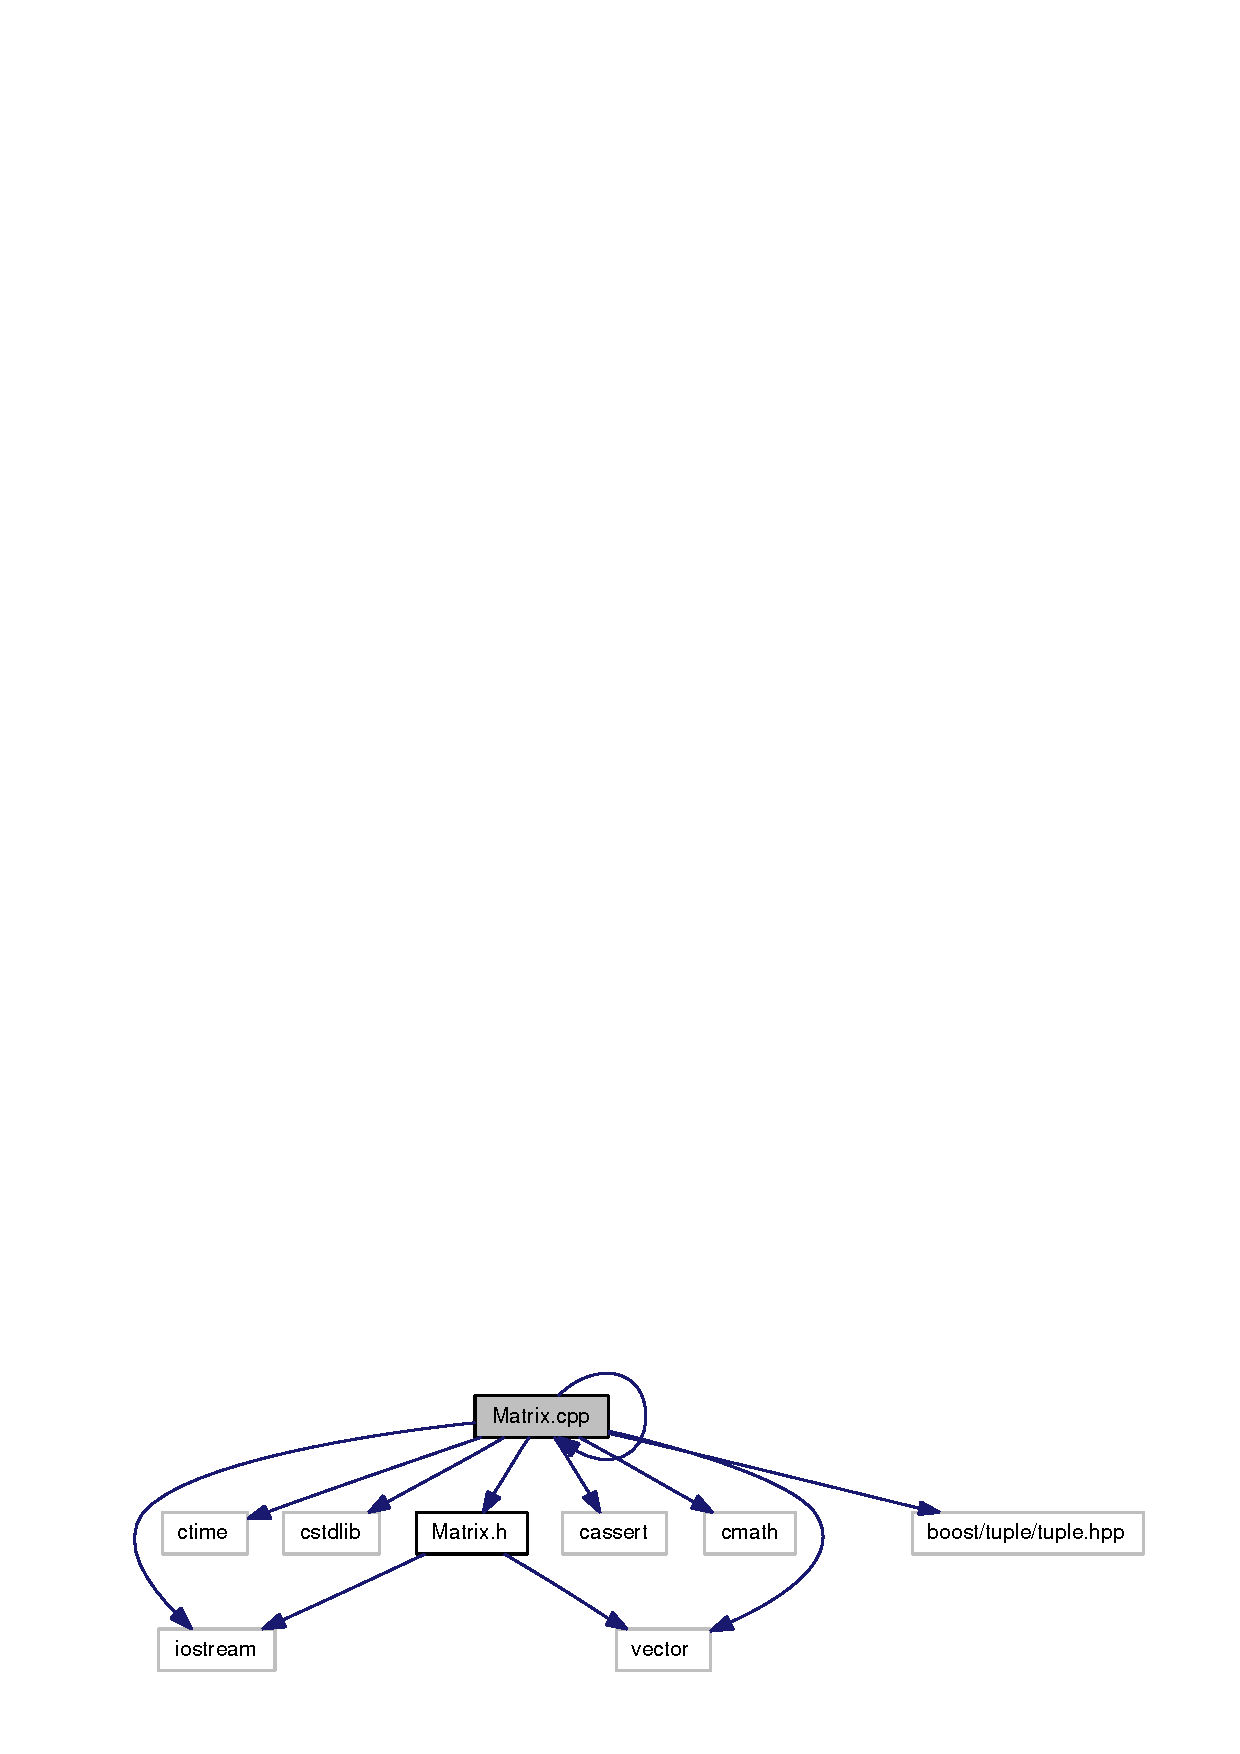
\includegraphics[width=276pt]{_matrix_8cpp__incl}
\end{center}
\end{figure}
This graph shows which files directly or indirectly include this file:\nopagebreak
\begin{figure}[H]
\begin{center}
\leavevmode
\includegraphics[width=63pt]{_matrix_8cpp__dep__incl}
\end{center}
\end{figure}
\subsection*{Functions}
\begin{DoxyCompactItemize}
\item 
\hyperlink{class_matrix}{Matrix} \& \hyperlink{_matrix_8cpp_aef0abd0dfab7b317c00f847ea7673842}{operator$\ast$} (\hyperlink{class_matrix}{Matrix} \&a, \hyperlink{class_matrix}{Matrix} \&b)
\begin{DoxyCompactList}\small\item\em Multiplies two matrices and returns the resulting \hyperlink{class_matrix}{Matrix} object. \item\end{DoxyCompactList}\item 
\hyperlink{class_matrix}{Matrix} \& \hyperlink{_matrix_8cpp_accade08db7bbcb399bf0f7f6fc0f7a38}{operator$\ast$} (double s, \hyperlink{class_matrix}{Matrix} \&a)
\begin{DoxyCompactList}\small\item\em Multiplies a \hyperlink{class_matrix}{Matrix} object by a scalar (double) and returns the resulting \hyperlink{class_matrix}{Matrix} object. \item\end{DoxyCompactList}\item 
\hyperlink{class_matrix}{Matrix} \& \hyperlink{_matrix_8cpp_aab165f42146537ca4960efd0e1c2975c}{operator$\ast$} (\hyperlink{class_matrix}{Matrix} \&a, double s)
\begin{DoxyCompactList}\small\item\em Multiplies a \hyperlink{class_matrix}{Matrix} object by a scalar (double) and returns the resulting \hyperlink{class_matrix}{Matrix} object. \item\end{DoxyCompactList}\item 
\hyperlink{class_matrix}{Matrix} \& \hyperlink{_matrix_8cpp_a3e861c2a1976635b49ded957b0fc1de1}{operator+} (\hyperlink{class_matrix}{Matrix} \&a, \hyperlink{class_matrix}{Matrix} \&b)
\begin{DoxyCompactList}\small\item\em Adds two \hyperlink{class_matrix}{Matrix} objects elementwise and returns the resulting \hyperlink{class_matrix}{Matrix} object. \item\end{DoxyCompactList}\item 
\hyperlink{class_matrix}{Matrix} \& \hyperlink{_matrix_8cpp_a3c8b27309dc425642323ec213fbce7aa}{operator-\/} (\hyperlink{class_matrix}{Matrix} \&a, \hyperlink{class_matrix}{Matrix} \&b)
\begin{DoxyCompactList}\small\item\em Subtracts the second matrix from the first matrix returns the resulting \hyperlink{class_matrix}{Matrix} object. \item\end{DoxyCompactList}\item 
ostream \& \hyperlink{_matrix_8cpp_ae88f31e57329a153343a5f1fb714c88f}{operator$<$$<$} (ostream \&s, \hyperlink{class_matrix}{Matrix} \&m)
\item 
bool \hyperlink{_matrix_8cpp_a521b4fbb24969f12c91690fdada71daa}{operator==} (\hyperlink{class_matrix}{Matrix} \&a, \hyperlink{class_matrix}{Matrix} \&b)
\begin{DoxyCompactList}\small\item\em Tests if two \hyperlink{class_matrix}{Matrix} objects are equivalent. \item\end{DoxyCompactList}\end{DoxyCompactItemize}


\subsection{Function Documentation}
\hypertarget{_matrix_8cpp_aab165f42146537ca4960efd0e1c2975c}{
\index{Matrix.cpp@{Matrix.cpp}!operator$\ast$@{operator$\ast$}}
\index{operator$\ast$@{operator$\ast$}!Matrix.cpp@{Matrix.cpp}}
\subsubsection[{operator$\ast$}]{\setlength{\rightskip}{0pt plus 5cm}{\bf Matrix} \& operator$\ast$ ({\bf Matrix} \& {\em a}, \/  double {\em s})}}
\label{_matrix_8cpp_aab165f42146537ca4960efd0e1c2975c}


Multiplies a \hyperlink{class_matrix}{Matrix} object by a scalar (double) and returns the resulting \hyperlink{class_matrix}{Matrix} object. 

\hypertarget{_matrix_8cpp_accade08db7bbcb399bf0f7f6fc0f7a38}{
\index{Matrix.cpp@{Matrix.cpp}!operator$\ast$@{operator$\ast$}}
\index{operator$\ast$@{operator$\ast$}!Matrix.cpp@{Matrix.cpp}}
\subsubsection[{operator$\ast$}]{\setlength{\rightskip}{0pt plus 5cm}{\bf Matrix} \& operator$\ast$ (double {\em s}, \/  {\bf Matrix} \& {\em a})}}
\label{_matrix_8cpp_accade08db7bbcb399bf0f7f6fc0f7a38}


Multiplies a \hyperlink{class_matrix}{Matrix} object by a scalar (double) and returns the resulting \hyperlink{class_matrix}{Matrix} object. 

\hypertarget{_matrix_8cpp_aef0abd0dfab7b317c00f847ea7673842}{
\index{Matrix.cpp@{Matrix.cpp}!operator$\ast$@{operator$\ast$}}
\index{operator$\ast$@{operator$\ast$}!Matrix.cpp@{Matrix.cpp}}
\subsubsection[{operator$\ast$}]{\setlength{\rightskip}{0pt plus 5cm}{\bf Matrix} \& operator$\ast$ ({\bf Matrix} \& {\em a}, \/  {\bf Matrix} \& {\em b})}}
\label{_matrix_8cpp_aef0abd0dfab7b317c00f847ea7673842}


Multiplies two matrices and returns the resulting \hyperlink{class_matrix}{Matrix} object. 

\hypertarget{_matrix_8cpp_a3e861c2a1976635b49ded957b0fc1de1}{
\index{Matrix.cpp@{Matrix.cpp}!operator+@{operator+}}
\index{operator+@{operator+}!Matrix.cpp@{Matrix.cpp}}
\subsubsection[{operator+}]{\setlength{\rightskip}{0pt plus 5cm}{\bf Matrix} \& operator+ ({\bf Matrix} \& {\em a}, \/  {\bf Matrix} \& {\em b})}}
\label{_matrix_8cpp_a3e861c2a1976635b49ded957b0fc1de1}


Adds two \hyperlink{class_matrix}{Matrix} objects elementwise and returns the resulting \hyperlink{class_matrix}{Matrix} object. 

\hypertarget{_matrix_8cpp_a3c8b27309dc425642323ec213fbce7aa}{
\index{Matrix.cpp@{Matrix.cpp}!operator-\/@{operator-\/}}
\index{operator-\/@{operator-\/}!Matrix.cpp@{Matrix.cpp}}
\subsubsection[{operator-\/}]{\setlength{\rightskip}{0pt plus 5cm}{\bf Matrix} \& operator-\/ ({\bf Matrix} \& {\em a}, \/  {\bf Matrix} \& {\em b})}}
\label{_matrix_8cpp_a3c8b27309dc425642323ec213fbce7aa}


Subtracts the second matrix from the first matrix returns the resulting \hyperlink{class_matrix}{Matrix} object. 

\hypertarget{_matrix_8cpp_ae88f31e57329a153343a5f1fb714c88f}{
\index{Matrix.cpp@{Matrix.cpp}!operator$<$$<$@{operator$<$$<$}}
\index{operator$<$$<$@{operator$<$$<$}!Matrix.cpp@{Matrix.cpp}}
\subsubsection[{operator$<$$<$}]{\setlength{\rightskip}{0pt plus 5cm}ostream\& operator$<$$<$ (ostream \& {\em s}, \/  {\bf Matrix} \& {\em m})}}
\label{_matrix_8cpp_ae88f31e57329a153343a5f1fb714c88f}
\hypertarget{_matrix_8cpp_a521b4fbb24969f12c91690fdada71daa}{
\index{Matrix.cpp@{Matrix.cpp}!operator==@{operator==}}
\index{operator==@{operator==}!Matrix.cpp@{Matrix.cpp}}
\subsubsection[{operator==}]{\setlength{\rightskip}{0pt plus 5cm}bool operator== ({\bf Matrix} \& {\em a}, \/  {\bf Matrix} \& {\em b})}}
\label{_matrix_8cpp_a521b4fbb24969f12c91690fdada71daa}


Tests if two \hyperlink{class_matrix}{Matrix} objects are equivalent. 


\hypertarget{_matrix_8h}{
\section{Matrix.h File Reference}
\label{_matrix_8h}\index{Matrix.h@{Matrix.h}}
}


This file contains the declarations of the basic Linear Algebra classes and some methods that operate on them.  


{\ttfamily \#include $<$iostream$>$}\par
{\ttfamily \#include $<$vector$>$}\par
{\ttfamily \#include $<$boost/iterator/iterator\_\-facade.hpp$>$}\par
Include dependency graph for Matrix.h:\nopagebreak
\begin{figure}[H]
\begin{center}
\leavevmode
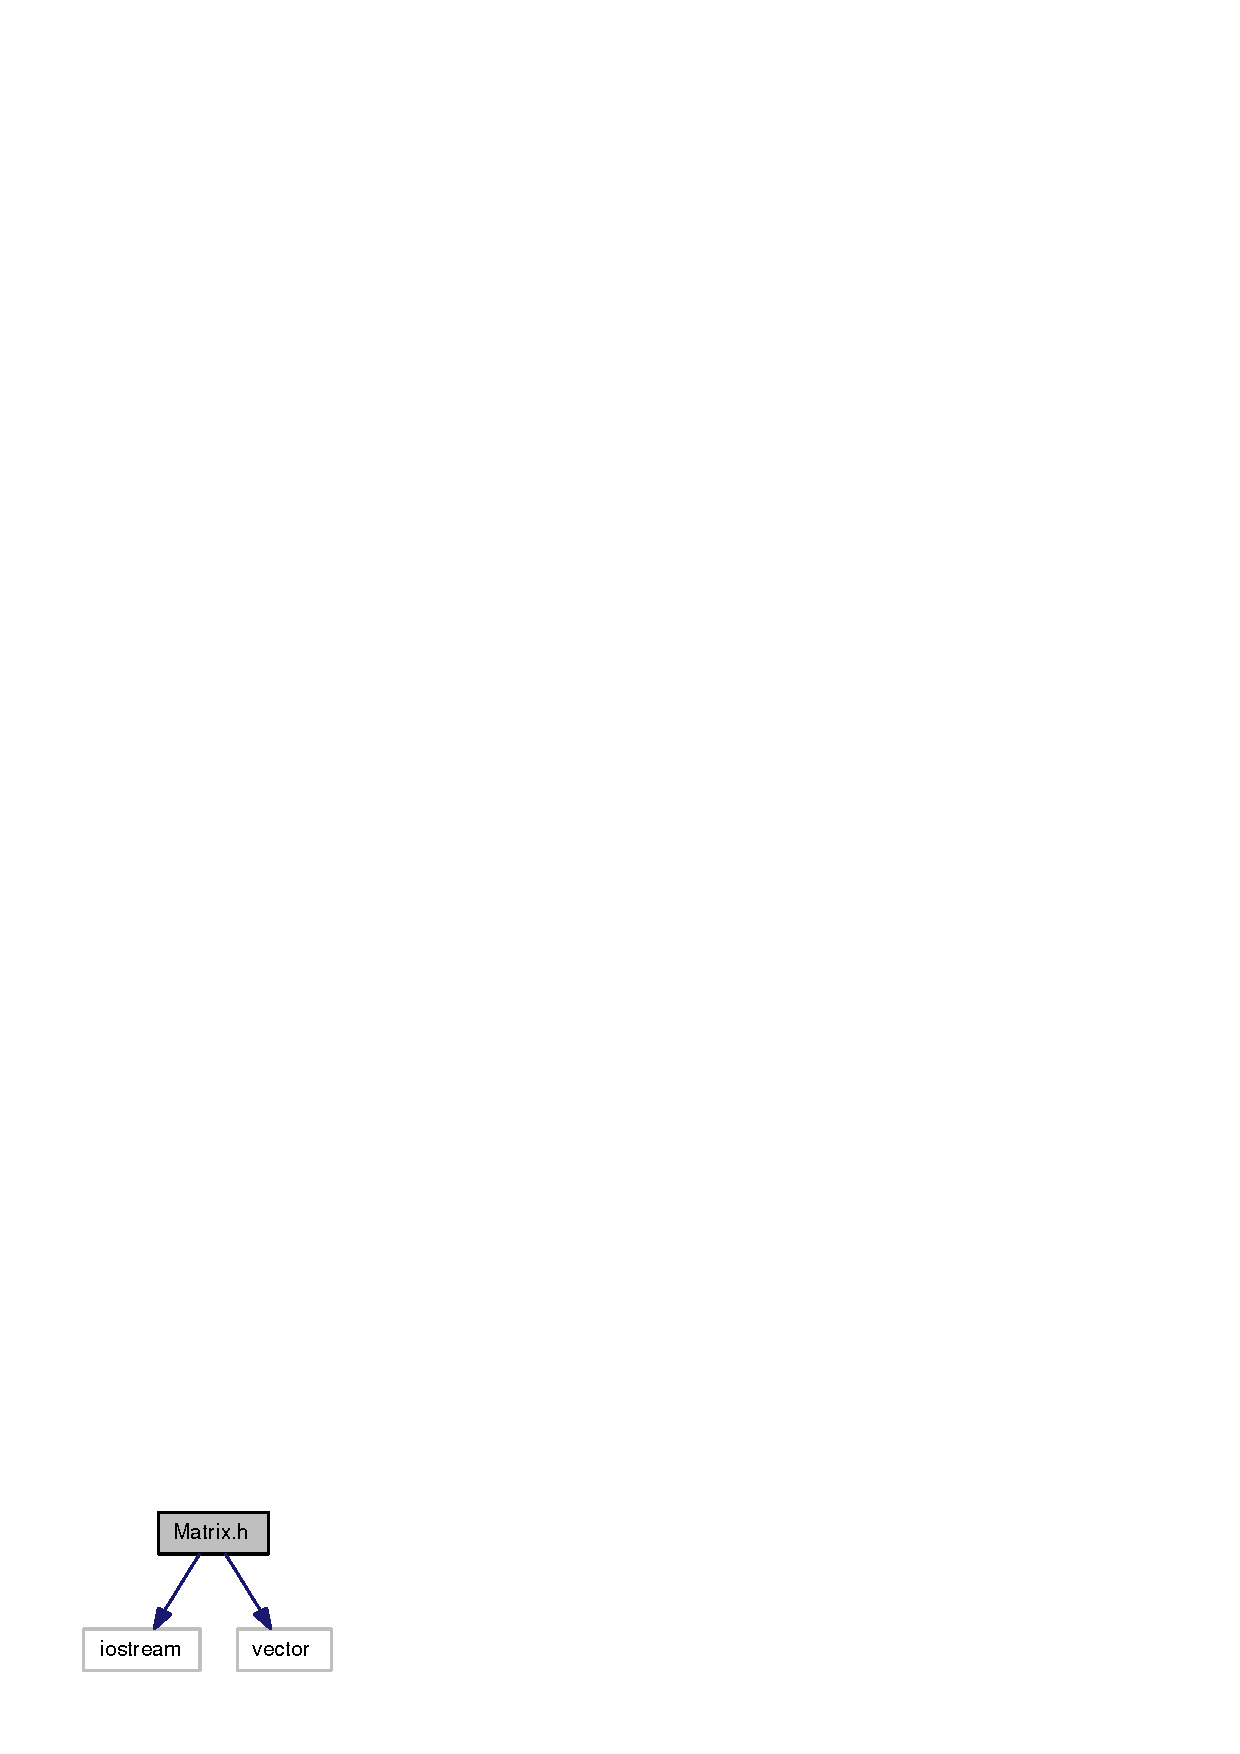
\includegraphics[width=174pt]{_matrix_8h__incl}
\end{center}
\end{figure}
This graph shows which files directly or indirectly include this file:\nopagebreak
\begin{figure}[H]
\begin{center}
\leavevmode
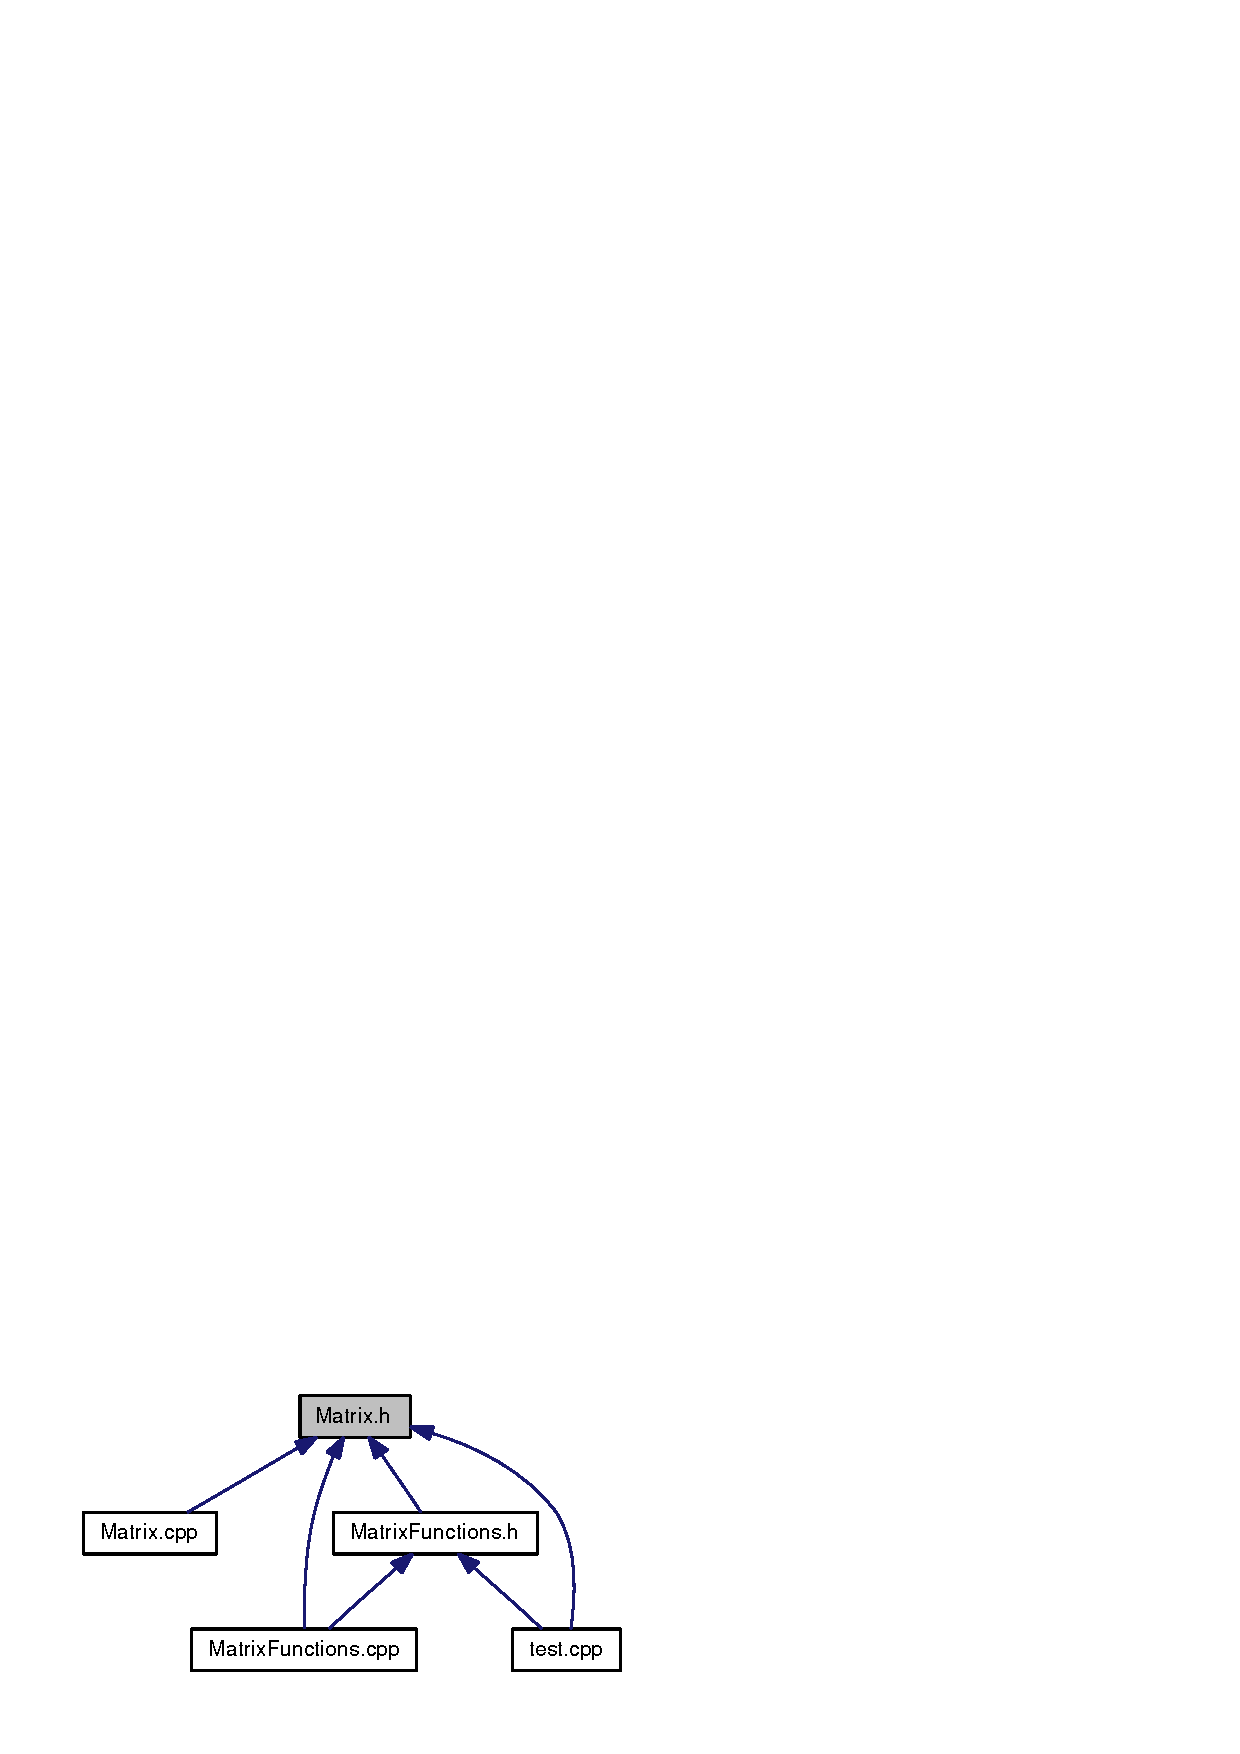
\includegraphics[width=160pt]{_matrix_8h__dep__incl}
\end{center}
\end{figure}
\subsection*{Classes}
\begin{DoxyCompactItemize}
\item 
class \hyperlink{class_matrix}{Matrix}
\begin{DoxyCompactList}\small\item\em The general \hyperlink{class_matrix}{Matrix} class. \item\end{DoxyCompactList}\item 
class \hyperlink{class_row_vector}{RowVector}
\begin{DoxyCompactList}\small\item\em The \hyperlink{class_row_vector}{RowVector} class, which inherits from the general \hyperlink{class_matrix}{Matrix} class. \item\end{DoxyCompactList}\item 
class \hyperlink{class_column_vector}{ColumnVector}
\begin{DoxyCompactList}\small\item\em The \hyperlink{class_column_vector}{ColumnVector} class, which inherits from the general \hyperlink{class_matrix}{Matrix} class. \item\end{DoxyCompactList}\item 
class \hyperlink{class_matrix_iterator}{MatrixIterator}
\begin{DoxyCompactList}\small\item\em The \hyperlink{class_matrix_iterator}{MatrixIterator} class. \item\end{DoxyCompactList}\end{DoxyCompactItemize}
\subsection*{Functions}
\begin{DoxyCompactItemize}
\item 
static const \hyperlink{class_matrix}{Matrix} \hyperlink{_matrix_8h_ac3e7400b224d99a4b9b96247c5912dfc}{NullMatrix} (0, 0)
\begin{DoxyCompactList}\small\item\em The NullMatrix is a special type of \hyperlink{class_matrix}{Matrix} with zero rows and zero columns. \item\end{DoxyCompactList}\item 
\hyperlink{class_matrix}{Matrix} \hyperlink{_matrix_8h_ab0bbb2ec9c1451f42f0270652df8cada}{operator$\ast$} (const \hyperlink{class_matrix}{Matrix} \&a, const \hyperlink{class_matrix}{Matrix} \&b)
\begin{DoxyCompactList}\small\item\em Multiplies two matrices and returns the resulting \hyperlink{class_matrix}{Matrix} object. \item\end{DoxyCompactList}\item 
\hyperlink{class_matrix}{Matrix} \hyperlink{_matrix_8h_a66de46fb456158acf519af331ff19038}{operator$\ast$} (const double s, const \hyperlink{class_matrix}{Matrix} \&a)
\begin{DoxyCompactList}\small\item\em Multiplies a \hyperlink{class_matrix}{Matrix} object by a scalar (double) and returns the resulting \hyperlink{class_matrix}{Matrix} object. \item\end{DoxyCompactList}\item 
\hyperlink{class_matrix}{Matrix} \hyperlink{_matrix_8h_a7f8bad991fbd1deff94dd1d54134ef32}{operator$\ast$} (const \hyperlink{class_matrix}{Matrix} \&a, const double s)
\begin{DoxyCompactList}\small\item\em Multiplies a \hyperlink{class_matrix}{Matrix} object by a scalar (double) and returns the resulting \hyperlink{class_matrix}{Matrix} object. \item\end{DoxyCompactList}\item 
\hyperlink{class_matrix}{Matrix} \hyperlink{_matrix_8h_ac6d5290381d2afbc2628dacbbacf0a34}{operator+} (const \hyperlink{class_matrix}{Matrix} \&a, const \hyperlink{class_matrix}{Matrix} \&b)
\begin{DoxyCompactList}\small\item\em Adds two \hyperlink{class_matrix}{Matrix} objects elementwise and returns the resulting \hyperlink{class_matrix}{Matrix} object. \item\end{DoxyCompactList}\item 
\hyperlink{class_matrix}{Matrix} \hyperlink{_matrix_8h_a21483b661257edc5f15dbbe7f88e8d84}{operator-\/} (const \hyperlink{class_matrix}{Matrix} \&a, const \hyperlink{class_matrix}{Matrix} \&b)
\begin{DoxyCompactList}\small\item\em Subtracts the second matrix from the first matrix returns the resulting \hyperlink{class_matrix}{Matrix} object. \item\end{DoxyCompactList}\item 
std::ostream \& \hyperlink{_matrix_8h_aa65f7cc3f08174c421a0b6d24dff90f1}{operator$<$$<$} (std::ostream \&s, const \hyperlink{class_matrix}{Matrix} \&m)
\begin{DoxyCompactList}\small\item\em Prints out a \hyperlink{class_matrix}{Matrix} object. \item\end{DoxyCompactList}\item 
bool \hyperlink{_matrix_8h_add6a39962db51ad24ca0c368177ff888}{operator==} (const \hyperlink{class_matrix}{Matrix} \&a, const \hyperlink{class_matrix}{Matrix} \&b)
\begin{DoxyCompactList}\small\item\em Tests if two \hyperlink{class_matrix}{Matrix} objects are equivalent. \item\end{DoxyCompactList}\end{DoxyCompactItemize}


\subsection{Detailed Description}
This file contains the declarations of the basic Linear Algebra classes and some methods that operate on them. 

\subsection{Function Documentation}
\hypertarget{_matrix_8h_ac3e7400b224d99a4b9b96247c5912dfc}{
\index{Matrix.h@{Matrix.h}!NullMatrix@{NullMatrix}}
\index{NullMatrix@{NullMatrix}!Matrix.h@{Matrix.h}}
\subsubsection[{NullMatrix}]{\setlength{\rightskip}{0pt plus 5cm}static const {\bf Matrix} NullMatrix (0, \/  0)\hspace{0.3cm}{\ttfamily  \mbox{[}static\mbox{]}}}}
\label{_matrix_8h_ac3e7400b224d99a4b9b96247c5912dfc}


The NullMatrix is a special type of \hyperlink{class_matrix}{Matrix} with zero rows and zero columns. 

If a function is supposed to return a \hyperlink{class_matrix}{Matrix} object, but an error has occured and it can't return the proper object, it should return a \hyperlink{class_matrix}{Matrix} with zero rows and zero columns by saying:


\begin{DoxyCode}
    return new Matrix(0,0);
\end{DoxyCode}


The return type should be compared with NullMatrix. For example, gaussJordan and gaussianElimination both return a \hyperlink{class_matrix}{Matrix} with zero rows and zero columns if no solution could be found; one way to use these functions would be:


\begin{DoxyCode}
    Matrix x = gaussianElimination(A,b); // where A and b are two previously defi
      ned matrices
    if (x == NullMatrix)
    {
        // uh oh!
    }else { ... }
\end{DoxyCode}
 \hypertarget{_matrix_8h_a7f8bad991fbd1deff94dd1d54134ef32}{
\index{Matrix.h@{Matrix.h}!operator$\ast$@{operator$\ast$}}
\index{operator$\ast$@{operator$\ast$}!Matrix.h@{Matrix.h}}
\subsubsection[{operator$\ast$}]{\setlength{\rightskip}{0pt plus 5cm}{\bf Matrix} operator$\ast$ (const {\bf Matrix} \& {\em a}, \/  const double {\em s})}}
\label{_matrix_8h_a7f8bad991fbd1deff94dd1d54134ef32}


Multiplies a \hyperlink{class_matrix}{Matrix} object by a scalar (double) and returns the resulting \hyperlink{class_matrix}{Matrix} object. 

\hypertarget{_matrix_8h_a66de46fb456158acf519af331ff19038}{
\index{Matrix.h@{Matrix.h}!operator$\ast$@{operator$\ast$}}
\index{operator$\ast$@{operator$\ast$}!Matrix.h@{Matrix.h}}
\subsubsection[{operator$\ast$}]{\setlength{\rightskip}{0pt plus 5cm}{\bf Matrix} operator$\ast$ (const double {\em s}, \/  const {\bf Matrix} \& {\em a})}}
\label{_matrix_8h_a66de46fb456158acf519af331ff19038}


Multiplies a \hyperlink{class_matrix}{Matrix} object by a scalar (double) and returns the resulting \hyperlink{class_matrix}{Matrix} object. 

\hypertarget{_matrix_8h_ab0bbb2ec9c1451f42f0270652df8cada}{
\index{Matrix.h@{Matrix.h}!operator$\ast$@{operator$\ast$}}
\index{operator$\ast$@{operator$\ast$}!Matrix.h@{Matrix.h}}
\subsubsection[{operator$\ast$}]{\setlength{\rightskip}{0pt plus 5cm}{\bf Matrix} operator$\ast$ (const {\bf Matrix} \& {\em a}, \/  const {\bf Matrix} \& {\em b})}}
\label{_matrix_8h_ab0bbb2ec9c1451f42f0270652df8cada}


Multiplies two matrices and returns the resulting \hyperlink{class_matrix}{Matrix} object. 

\hypertarget{_matrix_8h_ac6d5290381d2afbc2628dacbbacf0a34}{
\index{Matrix.h@{Matrix.h}!operator+@{operator+}}
\index{operator+@{operator+}!Matrix.h@{Matrix.h}}
\subsubsection[{operator+}]{\setlength{\rightskip}{0pt plus 5cm}{\bf Matrix} operator+ (const {\bf Matrix} \& {\em a}, \/  const {\bf Matrix} \& {\em b})}}
\label{_matrix_8h_ac6d5290381d2afbc2628dacbbacf0a34}


Adds two \hyperlink{class_matrix}{Matrix} objects elementwise and returns the resulting \hyperlink{class_matrix}{Matrix} object. 

\hypertarget{_matrix_8h_a21483b661257edc5f15dbbe7f88e8d84}{
\index{Matrix.h@{Matrix.h}!operator-\/@{operator-\/}}
\index{operator-\/@{operator-\/}!Matrix.h@{Matrix.h}}
\subsubsection[{operator-\/}]{\setlength{\rightskip}{0pt plus 5cm}{\bf Matrix} operator-\/ (const {\bf Matrix} \& {\em a}, \/  const {\bf Matrix} \& {\em b})}}
\label{_matrix_8h_a21483b661257edc5f15dbbe7f88e8d84}


Subtracts the second matrix from the first matrix returns the resulting \hyperlink{class_matrix}{Matrix} object. 

\hypertarget{_matrix_8h_aa65f7cc3f08174c421a0b6d24dff90f1}{
\index{Matrix.h@{Matrix.h}!operator$<$$<$@{operator$<$$<$}}
\index{operator$<$$<$@{operator$<$$<$}!Matrix.h@{Matrix.h}}
\subsubsection[{operator$<$$<$}]{\setlength{\rightskip}{0pt plus 5cm}std::ostream \& operator$<$$<$ (std::ostream \& {\em s}, \/  const {\bf Matrix} \& {\em m})}}
\label{_matrix_8h_aa65f7cc3f08174c421a0b6d24dff90f1}


Prints out a \hyperlink{class_matrix}{Matrix} object. 

\hypertarget{_matrix_8h_add6a39962db51ad24ca0c368177ff888}{
\index{Matrix.h@{Matrix.h}!operator==@{operator==}}
\index{operator==@{operator==}!Matrix.h@{Matrix.h}}
\subsubsection[{operator==}]{\setlength{\rightskip}{0pt plus 5cm}bool operator== (const {\bf Matrix} \& {\em a}, \/  const {\bf Matrix} \& {\em b})}}
\label{_matrix_8h_add6a39962db51ad24ca0c368177ff888}


Tests if two \hyperlink{class_matrix}{Matrix} objects are equivalent. 


\hypertarget{_matrix_functions_8cpp}{
\section{MatrixFunctions.cpp File Reference}
\label{_matrix_functions_8cpp}\index{MatrixFunctions.cpp@{MatrixFunctions.cpp}}
}
{\tt \#include \char`\"{}MatrixFunctions.h\char`\"{}}\par
{\tt \#include \char`\"{}Matrix.h\char`\"{}}\par


Include dependency graph for MatrixFunctions.cpp:\subsection*{Functions}
\begin{CompactItemize}
\item 
int \hyperlink{_matrix_functions_8cpp_a7678f1d5dfe64cad1897e1a78da2c10}{findNonZero} (\hyperlink{class_matrix}{Matrix} \&m, int col)
\begin{CompactList}\small\item\em Given a \hyperlink{class_matrix}{Matrix} and a column number, this functions returns the index of the first row which has a non-zero value in that column. \item\end{CompactList}\item 
\hyperlink{class_column_vector}{ColumnVector} \& \hyperlink{_matrix_functions_8cpp_e86ee38cefc33e331d995efa27d9cce2}{gaussJordan} (\hyperlink{class_matrix}{Matrix} \&A, \hyperlink{class_matrix}{Matrix} \&b)
\begin{CompactList}\small\item\em Given two matrices A and b, solves the linear system of equations assuming the form Ax = b. \item\end{CompactList}\item 
\hyperlink{class_column_vector}{ColumnVector} \& \hyperlink{_matrix_functions_8cpp_01929463f1c2846012d5ac2f1e1c1e4e}{gaussianElimination} (\hyperlink{class_matrix}{Matrix} \&A, \hyperlink{class_matrix}{Matrix} \&b)
\begin{CompactList}\small\item\em Given two matrices A and b, solves the linear system of equations assuming the form Ax = b. \item\end{CompactList}\end{CompactItemize}


\subsection{Function Documentation}
\hypertarget{_matrix_functions_8cpp_a7678f1d5dfe64cad1897e1a78da2c10}{
\index{MatrixFunctions.cpp@{MatrixFunctions.cpp}!findNonZero@{findNonZero}}
\index{findNonZero@{findNonZero}!MatrixFunctions.cpp@{MatrixFunctions.cpp}}
\subsubsection[{findNonZero}]{\setlength{\rightskip}{0pt plus 5cm}int findNonZero ({\bf Matrix} \& {\em m}, \/  int {\em col})}}
\label{_matrix_functions_8cpp_a7678f1d5dfe64cad1897e1a78da2c10}


Given a \hyperlink{class_matrix}{Matrix} and a column number, this functions returns the index of the first row which has a non-zero value in that column. 

If all rows have zeroes, it returns -1. This function is used by both gaussJordan and gaussianElimination. \hypertarget{_matrix_functions_8cpp_01929463f1c2846012d5ac2f1e1c1e4e}{
\index{MatrixFunctions.cpp@{MatrixFunctions.cpp}!gaussianElimination@{gaussianElimination}}
\index{gaussianElimination@{gaussianElimination}!MatrixFunctions.cpp@{MatrixFunctions.cpp}}
\subsubsection[{gaussianElimination}]{\setlength{\rightskip}{0pt plus 5cm}{\bf ColumnVector} \& gaussianElimination ({\bf Matrix} \& {\em A}, \/  {\bf Matrix} \& {\em b})}}
\label{_matrix_functions_8cpp_01929463f1c2846012d5ac2f1e1c1e4e}


Given two matrices A and b, solves the linear system of equations assuming the form Ax = b. 

Uses Gaussian Elimination with backsubstitution. Returns a \hyperlink{class_column_vector}{ColumnVector} object containing the solution. \hypertarget{_matrix_functions_8cpp_e86ee38cefc33e331d995efa27d9cce2}{
\index{MatrixFunctions.cpp@{MatrixFunctions.cpp}!gaussJordan@{gaussJordan}}
\index{gaussJordan@{gaussJordan}!MatrixFunctions.cpp@{MatrixFunctions.cpp}}
\subsubsection[{gaussJordan}]{\setlength{\rightskip}{0pt plus 5cm}{\bf ColumnVector} \& gaussJordan ({\bf Matrix} \& {\em A}, \/  {\bf Matrix} \& {\em b})}}
\label{_matrix_functions_8cpp_e86ee38cefc33e331d995efa27d9cce2}


Given two matrices A and b, solves the linear system of equations assuming the form Ax = b. 

Uses Gauss-Jordan. Returns a \hyperlink{class_column_vector}{ColumnVector} object containing the solution. 
\hypertarget{_matrix_functions_8h}{
\section{MatrixFunctions.h File Reference}
\label{_matrix_functions_8h}\index{MatrixFunctions.h@{MatrixFunctions.h}}
}


This file contains the declarations of the basic Linear Algebra classes and some methods that operate on them.  


{\ttfamily \#include $<$iostream$>$}\par
{\ttfamily \#include $<$vector$>$}\par
{\ttfamily \#include \char`\"{}Matrix.h\char`\"{}}\par
{\ttfamily \#include \char`\"{}boost/tuple/tuple.hpp\char`\"{}}\par
Include dependency graph for MatrixFunctions.h:\nopagebreak
\begin{figure}[H]
\begin{center}
\leavevmode
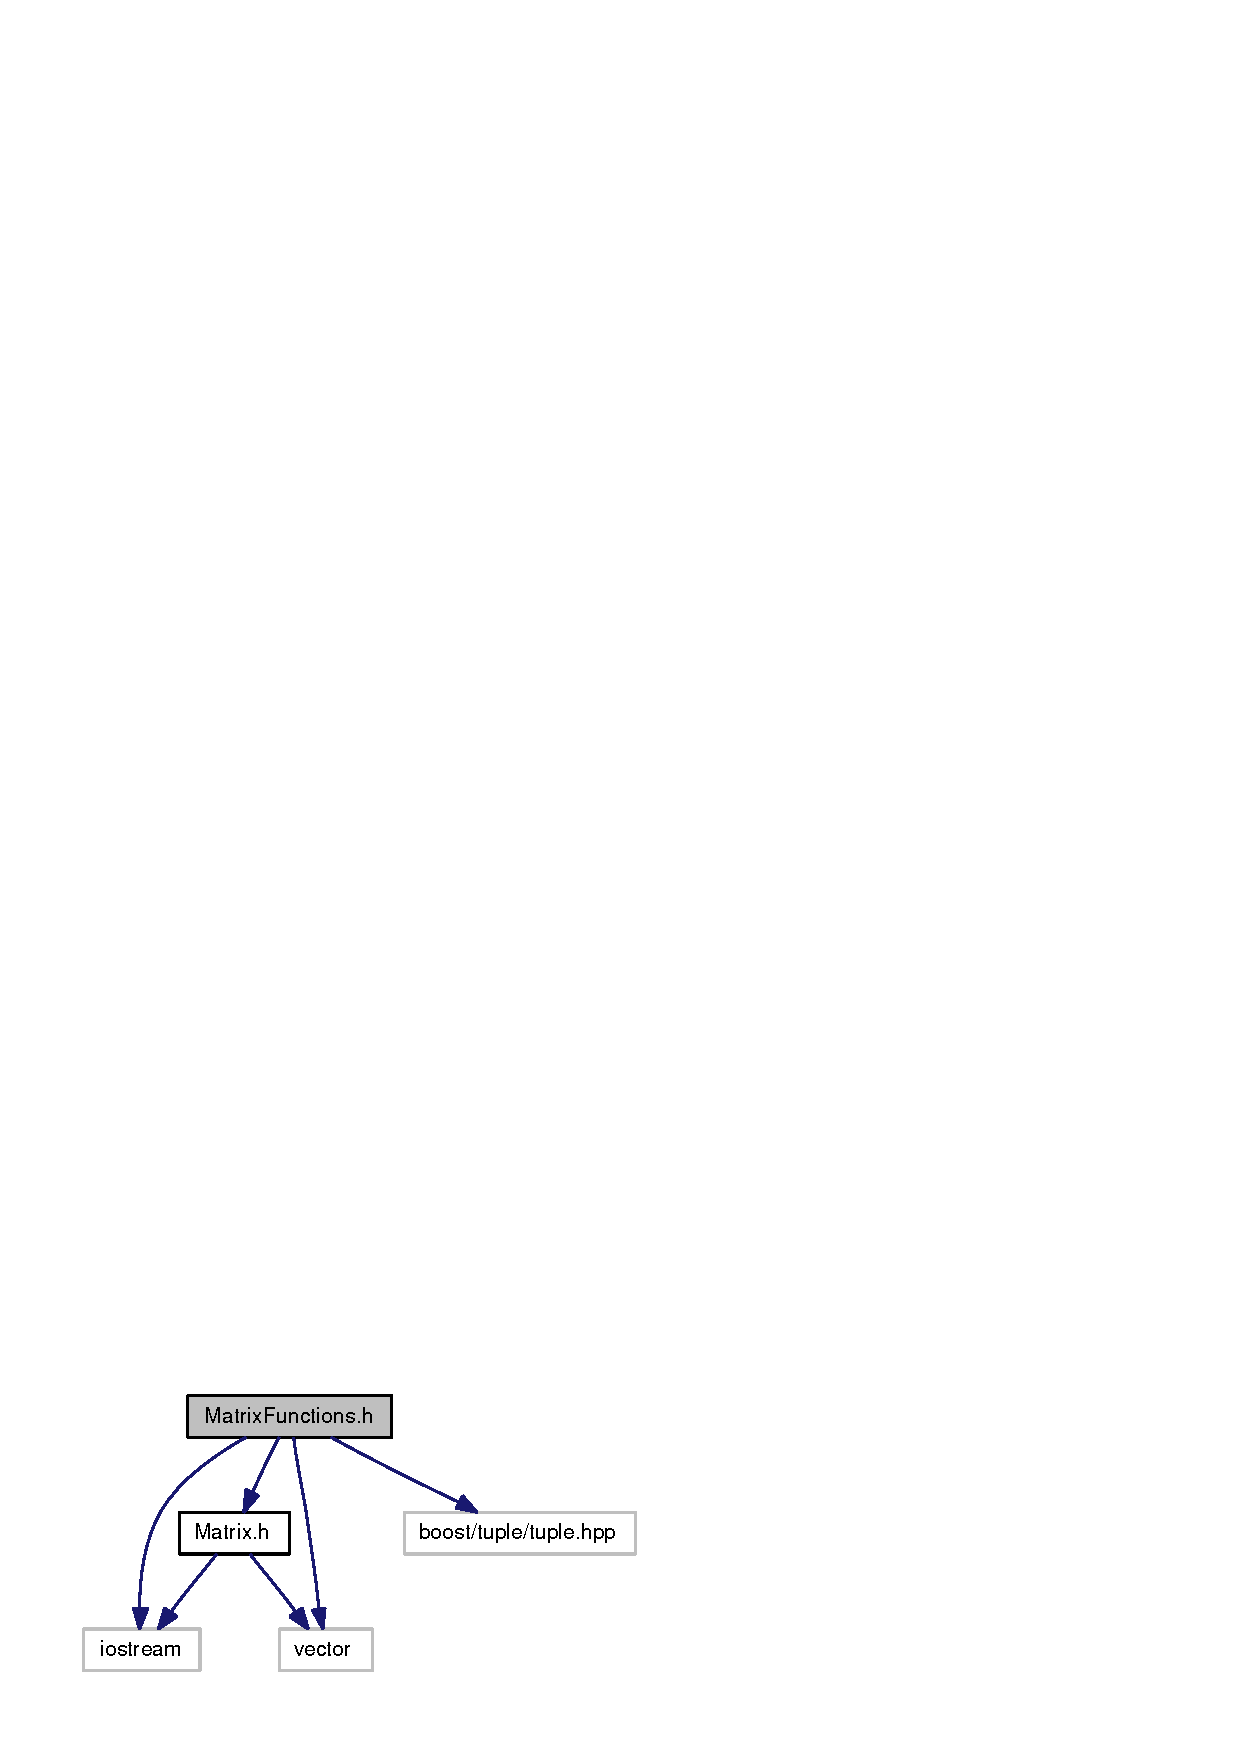
\includegraphics[width=197pt]{_matrix_functions_8h__incl}
\end{center}
\end{figure}
This graph shows which files directly or indirectly include this file:\nopagebreak
\begin{figure}[H]
\begin{center}
\leavevmode
\includegraphics[width=111pt]{_matrix_functions_8h__dep__incl}
\end{center}
\end{figure}
\subsection*{Functions}
\begin{DoxyCompactItemize}
\item 
int \hyperlink{_matrix_functions_8h_aa7678f1d5dfe64cad1897e1a78da2c10}{findNonZero} (\hyperlink{class_matrix}{Matrix} \&m, int col)
\begin{DoxyCompactList}\small\item\em Given a \hyperlink{class_matrix}{Matrix} and a column number, this functions returns the index of the first row which has a non-\/zero value in that column. \item\end{DoxyCompactList}\item 
\hyperlink{class_matrix}{Matrix} \hyperlink{_matrix_functions_8h_a566d910a6ada2d4c7d2eb602861bae9d}{gaussJordan} (\hyperlink{class_matrix}{Matrix} \&A, \hyperlink{class_matrix}{Matrix} \&b)
\begin{DoxyCompactList}\small\item\em Given two matrices A and b, solves the linear system of equations assuming the form Ax = b. \item\end{DoxyCompactList}\item 
\hyperlink{class_matrix}{Matrix} \hyperlink{_matrix_functions_8h_ae7079e2bd8e1e2bab782ab049b84cc45}{gaussianElimination} (\hyperlink{class_matrix}{Matrix} \&A, \hyperlink{class_matrix}{Matrix} \&b)
\begin{DoxyCompactList}\small\item\em Given two matrices A and b, solves the linear system of equations assuming the form Ax = b. \item\end{DoxyCompactList}\item 
boost::tuple$<$ \hyperlink{class_matrix}{Matrix}, \hyperlink{class_matrix}{Matrix}, \hyperlink{class_matrix}{Matrix} $>$ \hyperlink{_matrix_functions_8h_a3a79c07a22dd5e176404f713b54e5dfc}{LUPDecompose} (\hyperlink{class_matrix}{Matrix} A)
\begin{DoxyCompactList}\small\item\em Given a matrix, returns it's LUP decomposition. \item\end{DoxyCompactList}\item 
bool \hyperlink{_matrix_functions_8h_afd17d61898fe54cfb57b97238a20eab5}{isSymmetric} (\hyperlink{class_matrix}{Matrix} \&A)
\begin{DoxyCompactList}\small\item\em Checks whether a matrix is symmetric or not. \item\end{DoxyCompactList}\item 
\hyperlink{class_matrix}{Matrix} \hyperlink{_matrix_functions_8h_a0ad9f45bf1edd75781d68413d162cb0c}{steepestDescent} (\hyperlink{class_matrix}{Matrix} \&A, \hyperlink{class_matrix}{Matrix} \&b)
\begin{DoxyCompactList}\small\item\em Given two matrices A and b, solves the linear system of equations assuming the form Ax = b. \item\end{DoxyCompactList}\item 
\hyperlink{class_matrix}{Matrix} \hyperlink{_matrix_functions_8h_a12c19521809b4f556360bbea91aea576}{conjugateGradient} (\hyperlink{class_matrix}{Matrix} \&A, \hyperlink{class_matrix}{Matrix} \&b)
\begin{DoxyCompactList}\small\item\em Given two matrices A and b, solves the linear system of equations assuming the form Ax = b. \item\end{DoxyCompactList}\item 
\hyperlink{class_matrix}{Matrix} \hyperlink{_matrix_functions_8h_aaf686c3d17b6c76f2d79e291a31c2d02}{jacobi} (\hyperlink{class_matrix}{Matrix} \&A, \hyperlink{class_matrix}{Matrix} \&b)
\begin{DoxyCompactList}\small\item\em Given two matrices A and b, solves the linear system of equations assuming the form Ax = b. \item\end{DoxyCompactList}\end{DoxyCompactItemize}


\subsection{Detailed Description}
This file contains the declarations of the basic Linear Algebra classes and some methods that operate on them. 

\subsection{Function Documentation}
\hypertarget{_matrix_functions_8h_a12c19521809b4f556360bbea91aea576}{
\index{MatrixFunctions.h@{MatrixFunctions.h}!conjugateGradient@{conjugateGradient}}
\index{conjugateGradient@{conjugateGradient}!MatrixFunctions.h@{MatrixFunctions.h}}
\subsubsection[{conjugateGradient}]{\setlength{\rightskip}{0pt plus 5cm}{\bf Matrix} conjugateGradient ({\bf Matrix} \& {\em A}, \/  {\bf Matrix} \& {\em b})}}
\label{_matrix_functions_8h_a12c19521809b4f556360bbea91aea576}


Given two matrices A and b, solves the linear system of equations assuming the form Ax = b. 

Uses the Method of Conjugate Gradients. This is an iterative method. On sparse matrices, this will usually be faster than using gaussianElimination, gaussJordan and steepestDescent as well (it's a modified version of steepestDescent).

Warning: A needs to be symmetric and positive definite.

Returns a \hyperlink{class_matrix}{Matrix} object containing the solution. \hypertarget{_matrix_functions_8h_aa7678f1d5dfe64cad1897e1a78da2c10}{
\index{MatrixFunctions.h@{MatrixFunctions.h}!findNonZero@{findNonZero}}
\index{findNonZero@{findNonZero}!MatrixFunctions.h@{MatrixFunctions.h}}
\subsubsection[{findNonZero}]{\setlength{\rightskip}{0pt plus 5cm}int findNonZero ({\bf Matrix} \& {\em m}, \/  int {\em col})}}
\label{_matrix_functions_8h_aa7678f1d5dfe64cad1897e1a78da2c10}


Given a \hyperlink{class_matrix}{Matrix} and a column number, this functions returns the index of the first row which has a non-\/zero value in that column. 

If all rows have zeroes, it returns -\/1. This function is used by both gaussJordan and gaussianElimination. \hypertarget{_matrix_functions_8h_ae7079e2bd8e1e2bab782ab049b84cc45}{
\index{MatrixFunctions.h@{MatrixFunctions.h}!gaussianElimination@{gaussianElimination}}
\index{gaussianElimination@{gaussianElimination}!MatrixFunctions.h@{MatrixFunctions.h}}
\subsubsection[{gaussianElimination}]{\setlength{\rightskip}{0pt plus 5cm}{\bf Matrix} gaussianElimination ({\bf Matrix} \& {\em A}, \/  {\bf Matrix} \& {\em b})}}
\label{_matrix_functions_8h_ae7079e2bd8e1e2bab782ab049b84cc45}


Given two matrices A and b, solves the linear system of equations assuming the form Ax = b. 

Uses Gaussian Elimination with backsubstitution. This is faster than using gaussJordan. Returns a \hyperlink{class_matrix}{Matrix} object containing the solution. \hypertarget{_matrix_functions_8h_a566d910a6ada2d4c7d2eb602861bae9d}{
\index{MatrixFunctions.h@{MatrixFunctions.h}!gaussJordan@{gaussJordan}}
\index{gaussJordan@{gaussJordan}!MatrixFunctions.h@{MatrixFunctions.h}}
\subsubsection[{gaussJordan}]{\setlength{\rightskip}{0pt plus 5cm}{\bf Matrix} gaussJordan ({\bf Matrix} \& {\em A}, \/  {\bf Matrix} \& {\em b})}}
\label{_matrix_functions_8h_a566d910a6ada2d4c7d2eb602861bae9d}


Given two matrices A and b, solves the linear system of equations assuming the form Ax = b. 

Uses Gauss-\/Jordan. Returns a \hyperlink{class_matrix}{Matrix} object containing the solution. \hypertarget{_matrix_functions_8h_afd17d61898fe54cfb57b97238a20eab5}{
\index{MatrixFunctions.h@{MatrixFunctions.h}!isSymmetric@{isSymmetric}}
\index{isSymmetric@{isSymmetric}!MatrixFunctions.h@{MatrixFunctions.h}}
\subsubsection[{isSymmetric}]{\setlength{\rightskip}{0pt plus 5cm}bool isSymmetric ({\bf Matrix} \& {\em A})}}
\label{_matrix_functions_8h_afd17d61898fe54cfb57b97238a20eab5}


Checks whether a matrix is symmetric or not. 

\hypertarget{_matrix_functions_8h_aaf686c3d17b6c76f2d79e291a31c2d02}{
\index{MatrixFunctions.h@{MatrixFunctions.h}!jacobi@{jacobi}}
\index{jacobi@{jacobi}!MatrixFunctions.h@{MatrixFunctions.h}}
\subsubsection[{jacobi}]{\setlength{\rightskip}{0pt plus 5cm}{\bf Matrix} jacobi ({\bf Matrix} \& {\em A}, \/  {\bf Matrix} \& {\em b})}}
\label{_matrix_functions_8h_aaf686c3d17b6c76f2d79e291a31c2d02}


Given two matrices A and b, solves the linear system of equations assuming the form Ax = b. 

Uses the Jacobi Method. This is an iterative method.

Warning: A needs to be strictly or irreducibly diagonally dominant. Strict row diagonal dominance means that for each row, the absolute value of the diagonal term is greater than the sum of the absolute values of the other terms.

Returns a \hyperlink{class_matrix}{Matrix} object containing the solution. \hypertarget{_matrix_functions_8h_a3a79c07a22dd5e176404f713b54e5dfc}{
\index{MatrixFunctions.h@{MatrixFunctions.h}!LUPDecompose@{LUPDecompose}}
\index{LUPDecompose@{LUPDecompose}!MatrixFunctions.h@{MatrixFunctions.h}}
\subsubsection[{LUPDecompose}]{\setlength{\rightskip}{0pt plus 5cm}boost::tuple$<${\bf Matrix}, {\bf Matrix}, {\bf Matrix}$>$ LUPDecompose ({\bf Matrix} {\em A})}}
\label{_matrix_functions_8h_a3a79c07a22dd5e176404f713b54e5dfc}


Given a matrix, returns it's LUP decomposition. 

Three matrices L, U and P are returned as a boost tuple. Example usage: 
\begin{DoxyCode}
    #include "boost/tuple/tuple.hpp"

    // create a new matrix
    Matrix A(3,3);
    A.populateRandom();
  
    // get its decomposition
    boost::tuple<Matrix,Matrix,Matrix> lu = LUPDecompose(A);
    Matrix L = lu.get<0>();
    Matrix U = lu.get<1>();
    Matrix P = lu.get<2>();
    
    // print out matrices
    cout << L << endl;
    cout << U << endl;
    cout << P << endl;
\end{DoxyCode}
 \hypertarget{_matrix_functions_8h_a0ad9f45bf1edd75781d68413d162cb0c}{
\index{MatrixFunctions.h@{MatrixFunctions.h}!steepestDescent@{steepestDescent}}
\index{steepestDescent@{steepestDescent}!MatrixFunctions.h@{MatrixFunctions.h}}
\subsubsection[{steepestDescent}]{\setlength{\rightskip}{0pt plus 5cm}{\bf Matrix} steepestDescent ({\bf Matrix} \& {\em A}, \/  {\bf Matrix} \& {\em b})}}
\label{_matrix_functions_8h_a0ad9f45bf1edd75781d68413d162cb0c}


Given two matrices A and b, solves the linear system of equations assuming the form Ax = b. 

Uses the Method of Steepest Descent. This is an iterative method. On sparse matrices, this will usually be faster than using gaussianElimination or gaussJordan.

Warning: A needs to be symmetric and positive definite.

Returns a \hyperlink{class_matrix}{Matrix} object containing the solution. 
\hypertarget{test_8cpp}{
\section{test.cpp File Reference}
\label{test_8cpp}\index{test.cpp@{test.cpp}}
}
{\ttfamily \#include \char`\"{}Matrix.h\char`\"{}}\par
{\ttfamily \#include \char`\"{}MatrixFunctions.h\char`\"{}}\par
{\ttfamily \#include $<$iostream$>$}\par
{\ttfamily \#include $<$algorithm$>$}\par
{\ttfamily \#include $<$numeric$>$}\par
Include dependency graph for test.cpp:\nopagebreak
\begin{figure}[H]
\begin{center}
\leavevmode
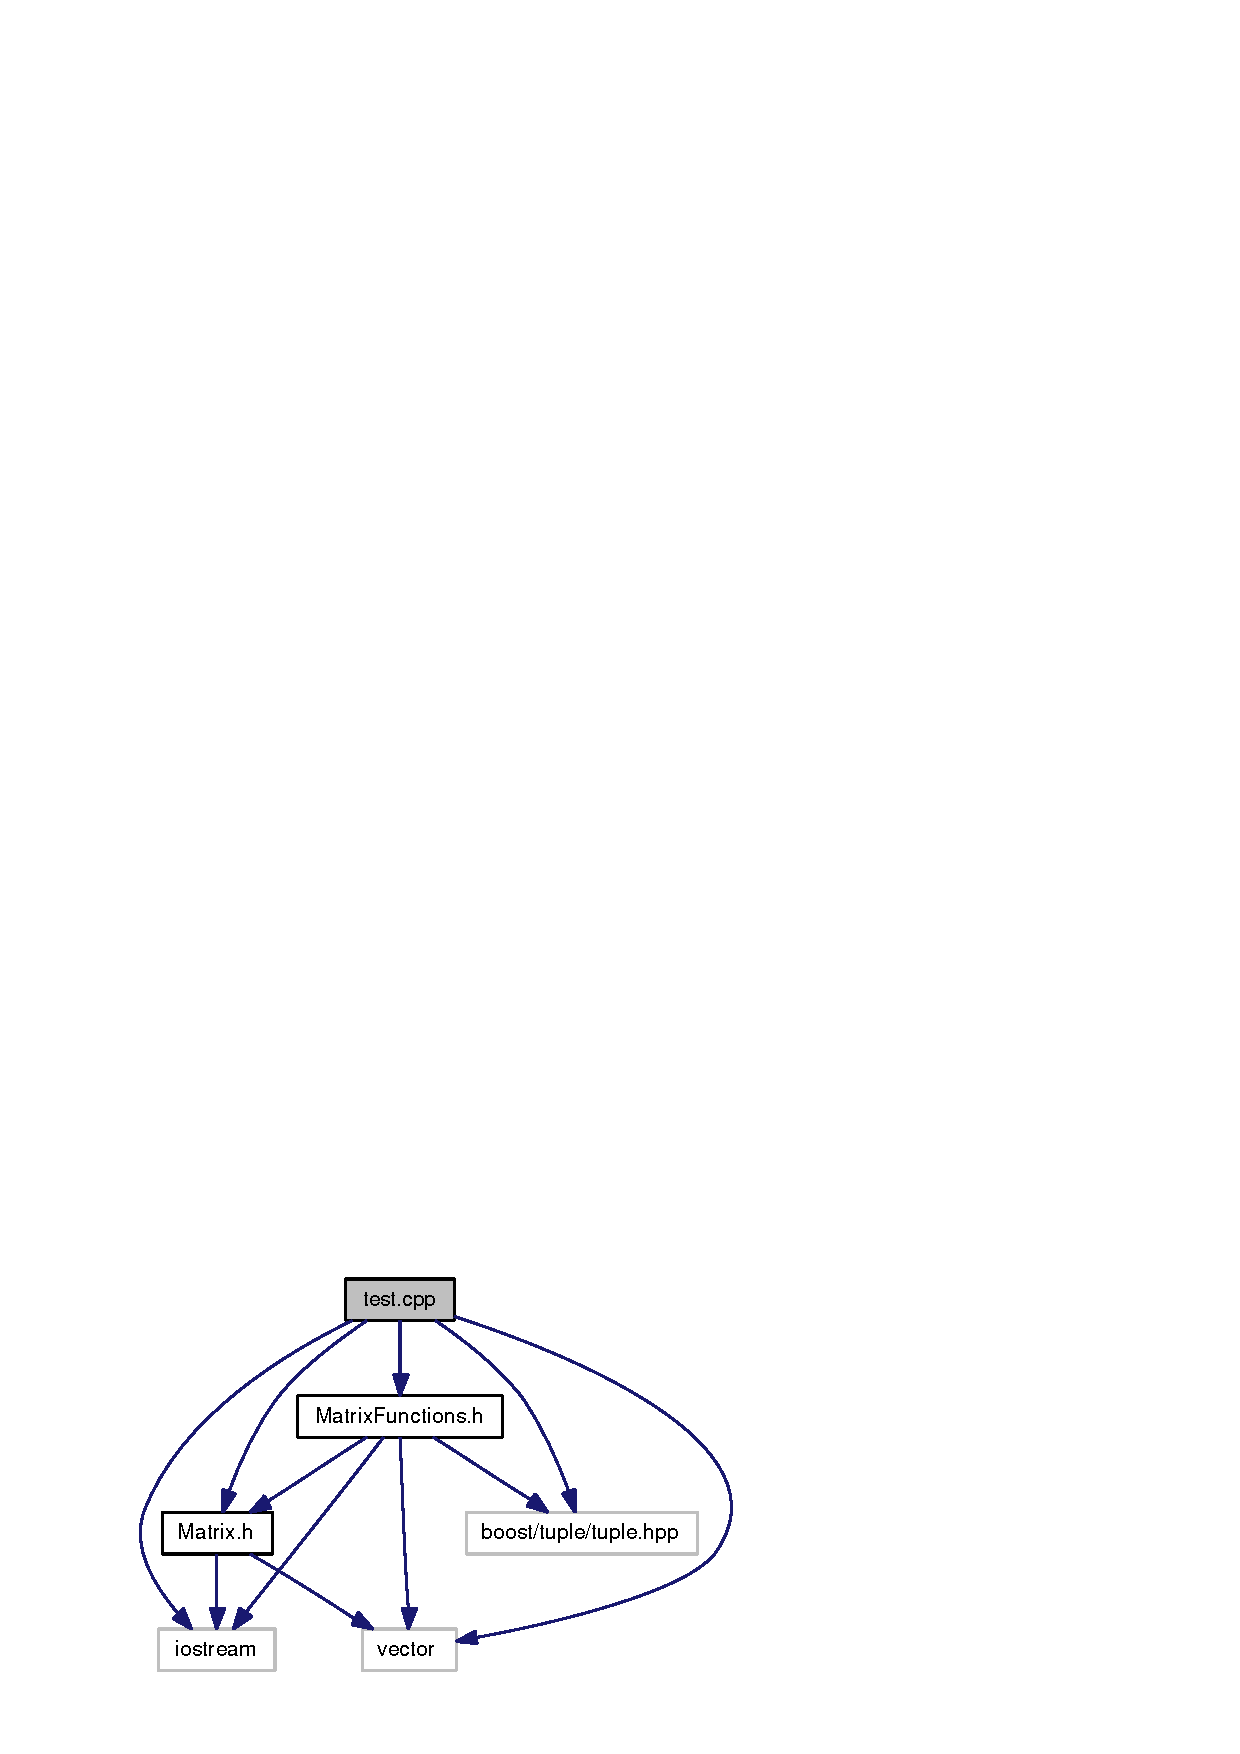
\includegraphics[width=208pt]{test_8cpp__incl}
\end{center}
\end{figure}
\subsection*{Functions}
\begin{DoxyCompactItemize}
\item 
int \hyperlink{test_8cpp_a0ddf1224851353fc92bfbff6f499fa97}{main} (int argc, char $\ast$argv\mbox{[}$\,$\mbox{]})
\end{DoxyCompactItemize}


\subsection{Function Documentation}
\hypertarget{test_8cpp_a0ddf1224851353fc92bfbff6f499fa97}{
\index{test.cpp@{test.cpp}!main@{main}}
\index{main@{main}!test.cpp@{test.cpp}}
\subsubsection[{main}]{\setlength{\rightskip}{0pt plus 5cm}int main (int {\em argc}, \/  char $\ast$ {\em argv}\mbox{[}$\,$\mbox{]})}}
\label{test_8cpp_a0ddf1224851353fc92bfbff6f499fa97}

\printindex
\end{document}
